%input "conext.bib"

%\documentclass[letterpaper,twocolumn,10pt]{article} % produces 14 pages
%\documentclass[]{acm_proc_article-sp} % produces 13 pages
\documentclass[letterpaper]{sig-alternate} % produces 12 pages
\sloppy

%\oddsidemargin  -0.24in
%\evensidemargin 0.0in
%\textwidth      6.99in
%\columnsep      0.33in
%\headheight     0.0in
%\topmargin      -0.6in
%\textheight     9.25in

\usepackage{subfigure}
\usepackage{epsfig}

%for PDF features - http://www.ce.cmu.edu/~kijoo/latex2pdf.pdf
\usepackage[pdftex,colorlinks]{hyperref} % For the bookmark/hyperlinks

\hypersetup{%
    pdftitle={Stealth Distributed Hash Table: A Robust and Flexible Super-Peered DHT},
    pdfauthor={Andrew Brampton, Andrew MacQuire, Idris A. Rai, Nicholas J. P. Race and Laurent Mathy},
    pdfkeywords={Distributed Hash Tables, Peer-to-Peer, Stealth DHT},
    bookmarksnumbered,
    pdfstartview={FitV},
    linkcolor={black},%: Color for normal internal links.
    anchorcolor={black},%: Color for anchor text.
    citecolor={black},%: Color for bibliographical citations in text.
    filecolor={black},%: Color for URLs which open local files.
    menucolor={black},%: Color for Acrobat menu items.
    pagecolor={black},%: Color for links to other pages
    urlcolor={black},%: Color for linked URLs.
}%

\author{
Andrew Brampton, Andrew MacQuire, Idris A. Rai,\\
Nicholas J. P. Race and Laurent Mathy\\
Computing Department,\\
Lancaster University\\
\{brampton,macquire,rai,race,laurent\}@comp.lancs.ac.uk
}
\date{}

\begin{document}

\title{Stealth Distributed Hash Table:\\A Robust and Flexible Super-Peered DHT}
\maketitle

\begin{abstract}
Most Distributed Hash Tables (DHTs) simply consider interconnecting {\em
homogeneous} nodes on the same overlay. However, realistically nodes on a
network are heterogeneous in terms of their capabilities. Because of this,
traditional DHTs have been shown to exhibit poor performance in a real-world
environment. Additionally, we believe that it is this approach that contributes
to a limited exploitation of peer-to-peer technologies. Previous work on
super-peers in DHTs was proposed to address these performance issues, however
the strategy used is often based on locally clustering peers around individual
super-peers. This method of super-peering, however, compromises fundamental
features such as load-balancing, resilience and routing efficiency, which
traditional DHTs originally promised to offer.

We propose a Stealth DHT which addresses the deficiencies of
previous super-peer approaches by using the DHT algorithm itself to
select the most appropriate super-peer for each message sent by
peers. Through simulations and measurements, we show the fitness for
purpose of our proposal.
\end{abstract}

% We might need to insert these
\category{C.2.1}{Computer-Communication Networks}{Network Architecture and Design}[Distributed networks]
\category{\\C.2.4}{Computer-Communication Networks}{Distributed Systems}

%General Terms: This section is limited to the following 16 terms:
% Algorithms, Management, Measurement, Documentation, Performance,
% Design, Economics, Reliability, Experimentation, Security, Human
% Factors, Standardization, Languages, Theory, Legal Aspects,
% Verification
\terms{Algorithms, Performance, Experimentation}

\keywords{Distributed Hash Tables, Peer-to-Peer, Stealth DHT}

%\CopyrightYear{2006}
%\crdata{� 2006 ACM  	1-59593-456-1/  	06/  	0012  	5.00}

~\\
\section{Introduction}
\label{sect-intro}

A common design approach for Distributed Hash Tables (DHTs) simply considers
interconnecting {\em autonomous} and {\em homogeneous} nodes on the same
overlay. The autonomicity of nodes arises in the sense that any node may join
or leave the network, and perform any operation supported by the DHT such as
{\em routing messages} or {\em putting} and {\em getting} data (indexed by {\em keys}) as they wish. On the other hand, the homogeneity of nodes assumes that nodes are equally capable devices which trust each other at the highest level.

Clearly, these assumptions are unrealistic for any practical large
scale network. This is demonstrated by various measurement studies
of peer-to-peer file sharing systems, which have shown a natural
inequality in the capabilities and behaviour of peers~\cite{sgg02}.
This leads to DHT based systems often operating at a level of
performance far below that which is expected. Indeed, lookup
latencies can be seriously affected by a node that has become a
routing bottleneck due to a lack of bandwidth or CPU cycles. Another
example is when nodes continually join and leave the network in an
unpredictable fashion, there can be tremendous increase in network
overhead. This behaviour is often referred to as \emph{churn},
severe levels of which have been shown to cause many DHTs to simply
break down~\cite{mobilechurn,dhtmanet01,churn1}.

A classical approach to improving this situation is to leverage the natural
heterogeneity in the system by using \emph{super-peers}~\cite{
mizrak03structured, zhu03superpeer}. However, most DHT-based super-peer
proposals rely on multiple overlays (\emph{e.g.} maintaining several rings) and
suffer from a rather static binding between peers and super-peers (\emph{i.e.}
the same super-peer proxies for peers' whole sessions). This, in turn, leads to
a higher maintenance overhead, as well as potentially single point of failure
and load-balancing issues.

In this paper we propose a simple, yet elegant technique applicable
to the majority of existing DHT systems, which enables the use of
super-peers in DHT-based networks, while avoiding the deficiencies
of previous super-peer approaches. Our proposal, the \emph{Stealth
Distributed Hash Table} (Stealth DHT), differs from traditional DHTs
mainly in that it makes a subset of nodes effectively ``invisible''
to the routing and forwarding decisions on the network. Therefore,
these nodes never receive any queries and thus cannot intercept nor
reply to them. As they are hidden from the rest of the overlay,
these nodes are referred to as \emph{stealth nodes}. In contrast,
the nodes responsible for forwarding messages in the DHT are
referred to as \emph{service nodes} (and are therefore equivalent to
super-peers). Salient features of a Stealth DHT are that it
maintains a single overlay, and that any source node (including
stealth nodes) uses the original routing decision process found in
traditional DHTs to choose the first hop of their message.  In other
words, the original DHT routing is used for super-peer selection on
a per message basis, meaning there exists no single point of failure
in the Stealth DHT approach -- preserving all of the benefits of
traditional DHTs whilst enabling super-peering.

Realistically, we envisage service nodes making up a relatively small
percentage of nodes in the DHT, perhaps owned by a single entity as a means of
service provision. It therefore follows that they should ideally be highly
stable and capable machines (\emph{e.g.} dedicated servers). Conversely,
stealth nodes are expected to be heterogeneous, autonomous devices owned by
end-users and are likely to connect and disconnect from the network in an
unpredictable fashion.

In this paper, we focus on evaluating the performance of Stealth DHTs
in comparison with a traditional DHT, both with and without churn in
the DHT population. While we believe that a Stealth DHT can be created
from almost any of the numerous existing algorithms to date, we chose
Pastry~\cite{rowstron01pastry} to be used in our performance
evaluation, as we deemed it to be a good representation of a typical
DHT. We later use both simulations and an implementation running on
PlanetLab~\cite{planetlab} to critically evaluate our approach. In
particular, we show how a Stealth DHT can reduce messaging overhead,
reduce object retrieval latency, provide greater resilience under churn
and more, all for the cost of increased load being placed on a small
number of (presumably over-provisioned) nodes.

The rest of the paper is organised as follows. In
Section~\ref{sect-overview}, we present a brief overview of
traditional DHT concepts, then continue by discussing the details of
a Stealth DHT in Section~\ref{sect-stealth}. We explain our
evaluation methodology and go on to show a number of results in
Section~\ref{sect-eval}. We then discuss potential applications of
the Stealth DHT work in Section~\ref{sect-applications}. Work
related to our proposal is elaborated upon in
Section~\ref{sect-related} and finally we conclude the paper in
Section~\ref{sect-conclusions}.

\section{DHT Overview}
\label{sect-overview}

Distributed Hash Tables (DHTs) have been shown to be a promising form of
decentralised structured peer-to-peer networking, offering substantial
scalability and resilience. Unsurprisingly, there exist numerous DHT
systems~\cite{rowstron01pastry,chord01,tapestry01,can01}. Primarily, DHTs serve
as an object location service that can be used as a substrate for multiple
large-scale distributed applications such as
storage~\cite{past,dabek01,oceanstore}, multicast~\cite{scribe,bayeux} and load
balancing systems~\cite{kar04,bri05}.

Many DHT algorithms have a similar structure, wherein each node on the network
has a unique identifier (ID), randomly generated within the address space. The
address space is dynamically partitioned into regions depending on the number
of nodes and their addresses. Each region is then assigned to a single node.

Each key in the DHT is generated by applying a hash function to the
object it represents, producing an identifier that falls within a
specific region of the address space.  The DHT algorithm ensures
that the key is held by the node responsible for that region.  In
most implementations a node will maintain relatively sparse routing
state spanning the entire address space, which will grow with
increasing numbers of nodes in the DHT.

A reference to an object can then be retrieved by sending a request
message addressed to the value of the corresponding key. The DHT
routing algorithm then ensures that this message is actually
delivered to the node responsible for the region of the address
space where the key falls.

When a new node joins a DHT, it must first initialise its routing
table. The assumption is made that the new node will know at least
one established node on the network. This \emph{bootstrap} node can
be used to route a {\em join} message to the region that the joining
node's ID lies within.

DHTs normally provide good routing performance in terms of average overlay
hops, varying slightly depending on the routing algorithm used. The actual
trend will often depend on the geometry of the DHT itself. For instance,
Pastry, Chord and Tapestry~\cite{rowstron01pastry, chord01, tapestry01} are all
based on the common ring structure, giving approximately $O(log N)$ hops, where
$N$ is the number of nodes in the DHT. Content Addressable Network
(CAN)~\cite{can01}, however, is a $d$-dimensional space, instead giving
(d/4)(N$^{1/d}$) hops on average.

The following section provides an overview of the Stealth DHT approach
based upon Pastry.

%%%%%%%%%%%%

\section{Stealth DHT Overview}
\label{sect-stealth}

A Stealth DHT differs from a traditional DHT in that it splits the network into
nodes of two differing types: \emph{service} and \emph{stealth}. Service nodes
are expected to be highly capable, reliable machines, and they provide the
routing infrastructure for the overlay. Stealth nodes are ``clients'' that
communicate with and through service nodes only. Note however, that the
assignment of role to nodes is application dependent and in no way prescribed
or constrained by the Stealth DHT itself. Future work may involve automatic
assignment of roles to nodes to improve the autonomicity of the system. This
paper concentrates on the modifications required for a Stealth Pastry DHT,
however we believe that similar simple general principles can be applied to
other DHTs too.

\begin{figure}[tb]\centering
\subfigure[State Gathering Phase]
    {\includegraphics[width=0.2\textwidth]{./diagrams/JoinA}
    \label{fig:phase1_pastry}}
\subfigure[Announcement Phase]
    {\includegraphics[width=0.2\textwidth]{./diagrams/JoinB}
    \label{fig:phase2_pastry}}
\caption{\em Join Procedure}
\label{fig:join_procedure}
\end{figure}

\subsection{Service Node Join}
\label{subsect-join:service}

A service node is a fully-fledged DHT node and joins the (Stealth)
DHT in conformance with the method prescribed by the original DHT.

It is worth noting that the join procedure in traditional DHTs conceptually has
two phases: a state gathering phase at the end of which the joining node will
have received enough information (routing, \emph{etc.}) to take part in the
DHT, and an announcement phase through which the joining node advertises its
presence on the overlay to some of the nodes already present.

% AB: This section was hard to read so I changed it a little but maybe made it a little unclear now
The state gathering phase in Pastry is depicted in
Fig.~\ref{fig:phase1_pastry}. Remember that a service node joins the network in
the same way a typical Pastry node would. A Pastry (or a service) node $X$ uses
prior knowledge of a bootstrap (service) node $A$ to route a join message into
the DHT, destined for the (service) node closest to $X$'s randomly generated
ID. Upon receiving and forwarding the message, (service) nodes $A$ and $B$ send
a relevant fraction of their routing table directly to $X$. The join message
then arrives at its destination $C$ (the closest (service) node to $X$'s ID).
$C$, in addition to sending routing data, informs $X$ about neighbourhood
information (\emph{i.e.} leafset) and that finishes the state gathering phase.
Node $X$ then proceeds with the announcement phase (see
Fig.~\ref{fig:phase2_pastry}) to announce its presence and ID on the ring to
some other (service) nodes. The main purpose of this announcement is to enable
the presence of $X$ in other nodes' routing tables.

\subsection{Stealth Node Join}
\label{subsect-join:stealth}

A stealth node joins the Stealth DHT by only completing the state gathering
phase of the original DHT, and ignoring the announcement phase. This is
illustrated in Fig.~\ref{fig:phase1_pastry}, but in this case node $X$ is a
stealth node and all other nodes depicted are service nodes. In particular, the
reader should note that the node used as bootstrap node should be a service
node.

The effect of not initiating any announcement phase is that no service
node ever learns to route through a stealth node. In other words, a
stealth node never appears in any routing table, yet a stealth node is
able to route messages into the DHT using the routing information it
acquired during the state gathering phase. Stealth nodes are therefore
capable of injecting messages into the DHT, choosing the first hop for
their messages from their routing table in the same way `normal' DHT
nodes do, but are never used to relay any message, nor will they ever
receive any message on the DHT (unless a message is sent directly to
them from a service node \emph{e.g.} a reply to a query). This results
in a single overlay (in our example case a single DHT ring) that
accommodates both the service and stealth nodes.
%(Fig.~\ref{fig:stealthdht}).

%\begin{figure}[tb]
%\centering \epsfig{file=./diagrams/StealthDHT, width=0.2\textwidth}
%\caption{\em Stealth DHT structure} \label{fig:stealthdht}
%\end{figure}

From a functional point of view, stealth nodes can publish and retrieve keys in and from the DHT respectively. These operations are achieved by sending simple put or get
messages. However, as stealth nodes never receive put messages, only service
nodes can store keys, conferring them the status of super-peers.

As stealth nodes never appear in routing tables, several stealth nodes may
inadvertently choose the same node ID without collisions being detected.
Likewise, a new service node could also choose the same node ID as an existing
stealth node without it being detected. The only detectable collisions
involving a stealth node are those occurring when a new stealth node chooses a
ID that already identifies an existing service node. This is because ID
collisions are detected when the join message destination's ID is the same as
the last hop's node ID. In such cases, a \emph{collision} message is returned
to the joining node instead of the \emph{finished} message. However, because
stealth nodes do not relay messages nor hold keys, their IDs are never required
to locate them on the DHT ring so that unresolved node ID collisions involving
stealth nodes do not pose any problem to the operation of the Stealth DHT. In
essence, stealth nodes only pick a node ID to gather routing information. Of
course, the detectable stealth node ID collisions can be resolved by having the
stealth node select a new ID and then issue a new stealth join message.

Note that stealth nodes have no way of detecting the presence of
other stealth nodes, while service nodes can only know of stealth
nodes through their recent activity, hence the name of our scheme
which exhibits enhanced privacy properties compared to the original
DHT. A further benefit is that the lack of announcement messages
cuts the overhead of joining stealth nodes significantly.

\subsection{Stealth Routing State}
\label{subsect-state}

Several observations can be made about the routing state needed by
stealth nodes. Firstly, the role of the leafset in Pastry is to
ensure that message routing always completes
correctly~\cite{rowstron01pastry}. However, since stealth nodes only
initiate routing of messages (by selecting the first hop), it is
clear that a stealth node does not need to maintain a leafset which
is only used to consistently determine the last hop.

Secondly, if node IDs are represented in base $2^b$, the routing table is
conceptually a $log_{2^b}N \times 2^b$ array, where $N$ is the size of the
address space. This is because the entries of row $n$ of any node $Z$ contain
references to nodes whose IDs share a common ID prefix of length $n$ digits,
and therefore it is impossible to have more than $log_{2^b}N$ digits in common.
The $n+1$ ID digit corresponds to column number of the entry, and again there
are only $2^b$ different digits.

The routing procedure for a node that needs to send / forward a message is to
select the row of its routing table corresponding to its prefix match with the
destination ID (the first row of the routing table is row $0$ corresponding to
no prefix match) and pick as a next hop the entry of the column corresponding
to the value of first (non-matching) digit of the destination ID. This ensures
that the next hop of the message shares a longer ID prefix with the destination
than the current node does (and is therefore closer to the destination). This
very concise and simplified description of the routing procedure is enough for
our discussion and we refer the reader to~\cite{rowstron01pastry} for further
details of Pastry routing.

If we observe that the probability for two randomly chosen IDs not to share any
prefix is $\frac{2^b - 1}{2^b}$, we see that in the vast majority of cases, the
initial sender of a message will use the first row of its routing table to
select the first routing hop. Indeed, in the typical case where $b = 4$ (IDs in
base 16), this situation occurs $15/16 = 93.75\%$ of the time. Recalling that
stealth nodes are always the origin of any messages they send through the DHT,
then it is obvious that reducing the routing information in stealth nodes to
the first row of the routing table will have very little impact on routing
performance while greatly reducing state overhead. In other words, the service
nodes that handle the join message for a stealth node should only provide such
node with routing information contained in the first row of their routing table
(as opposed to information from the full routing table). It is natural to
question the performance gain when stealth nodes use a single row routing table
(with at most $2^b$ nodes' IDs) compared to when they have a list of a random
$2^b$ nodes' IDs from existing service nodes. We discuss the benefits of using
the former in Section \ref{subsubsect-random}.

Lastly, from the above description of routing, it should be clear
that one column per row of the routing table contains an empty
entry: this is the column corresponding to the $n+1$ digit of the ID
of the node holding the routing table (\emph{i.e.} the node itself).
This is because the corresponding entry in row $n$ would then share
a prefix of length $n+1$ with the node, and should therefore belong
on the following row. For stealth nodes, which only have a single
row in their routing table, this would mean that there would be no
next hop entry for destinations whose IDs have the first digit equal
to that of the stealth node. The only way a stealth node could then
send toward such destinations would be to pick any other entry at
random from their routing table and let that node (which does not
share any prefix with the destination) decide on a more appropriate
next hop. To avoid such sub-optimal ``dog leg'' routes, we require
that stealth nodes do have an entry pointing to a node that share a
one-digit prefix with the stealth node ID in the otherwise empty
column entry. This ensures that a complete and valid routing table
at a stealth node will always provide a next hop that has at least a
one-digit prefix with the destination.

\subsection{Stealth Routing State Maintenance}
When a service node leaves the network, some stealth nodes will
inevitably have obsolete information for that node in their routing
tables. Complete disconnection, however, can only occur when all
service nodes in a stealth node's routing table have left the DHT.
Just like service nodes, a stealth node will detect a failed service
node in its routing table when it attempts to send a message to that
node, or through maintenance probes.

One problem that arises as a result of the isolation of stealth
nodes is that their routing tables are difficult to keep up to date.
To recap, stealth nodes never receive announcement messages from
newly arrived service nodes as they are not addressable on the DHT.
A new method is therefore required for maintaining routing state at
stealth nodes. We propose several possible approaches: {\em
rejoining}, {\em periodic polling} and {\em piggybacking}.

A stealth node could rejoin the Stealth DHT on a periodic basis. This can be
done without changing its chosen node ID and can even bootstrap through any
entry of its routing table.

Periodic polling is a variation of rejoining where a stealth node
periodically queries any of the service nodes in its routing table
for its current relevant routing state (as opposed to all the nodes
on the path to a service node closest to its ID).

The piggybacking approach requires service nodes to attach some additional
routing state to every message it sends to a stealth node\footnote{Recall that
although stealth nodes are not addressable on the DHT, a service node will
communicate directly via the underlying network with a stealth node when
responding to a solicitation from it.}. Upon receiving each message from a
service node, a stealth node checks these attached IDs to see if they can be
used to update its routing table. This approach allows the routing tables in
stealth nodes to stay fresh whilst being updated in a passive fashion. An added
benefit is that the mechanism is ``self-tuning'': the more active a stealth
node is on the network, the fresher and more complete its routing table is.

To evaluate the respective merits of these different approaches for refreshing
routing state in stealth nodes, we have run the same simulation scenario for
each, with varying rates of churn (refer to Section~\ref{sect-eval} for details
on the simulation setup). Fig.~\ref{fig:route_validity} shows the average
number of valid routing entries in stealth node routing tables (\emph{i.e.} one
row with $2^b$ entries where $b = 4$), while
Fig.~\ref{fig:route_validity_overhead} shows the overall number of messages
observed during the scenario (\emph{e.g.} queries, routing updates,
\emph{etc.}). Note that the period for polling was set to 100 seconds, while
that for rejoining to 5 minutes.

From these results, it seems clear that polling provides the best routing table
maintenance, albeit at the highest cost. This is due to two messages being
generated at each polling interval (the request and reply message). In
contrast, the rejoining mechanism updates state 3 times less frequently than
polling, but only generates $log_{2^b}N$ message per join. Overall,
piggybacking appears to offer a better accuracy versus cost tradeoff, as it
does not increase the number of messages (although it does slightly increase
the message size) while keeping the routing table fresh.

\begin{figure}[tb]\centering
\subfigure[Validity of routing entries]
    {\includegraphics[width=0.415\textwidth]{./diagrams/RecoveryValid}
    \label{fig:route_validity}}
\subfigure[Overhead]
    {\includegraphics[width=0.415\textwidth]{./diagrams/RecoveryMessages}
    \label{fig:route_validity_overhead}}
\caption{\em Stealth routing state refresh}
\label{fig:route_refresh}
\end{figure}

\section{Evaluation}
\label{sect-eval}

In order to evaluate our Stealth DHT proposal, we developed our own
discrete-event packet-level simulator for Pastry and Stealth DHTs, because
existing Pastry simulators did not offer all the features we required. We also
implemented both Pastry and a Stealth DHT for evaluation in a real-world
environment (PlanetLab). As with our simulator, we considered modifying an
existing open-source project such as FreePastry or
Bamboo~\cite{freepastry,churn1}, but found the flexibility of creating our own
implementation to be preferable.

Throughout the paper, we describe Stealth DHTs networks as
\emph{Stealth~($S$\%)}, where $S$\% of nodes on the DHT are stealth
nodes. For example, when we discuss the performance of a Stealth~(95\%)
DHT, it implies that 95\% of the existing nodes are stealth nodes
(\emph{e.g.} on a 1,000 node DHT, 950 stealth and 50 service nodes
would exist). This is a value used repeatedly throughout the paper, as
it clearly shows the differences that using a Stealth DHT can make;
with lower values, results have been found to tend towards that of the
corresponding Pastry DHT.

In both the simulator and the implementation, 1,000 or more randomly generated
keys were initially put into the network. Each key was assigned a popularity
ranking following a Zipf distribution with an $\alpha$ parameter of 1.2.
Whenever a node performs a \emph{get} operation, the probability of it choosing
a particular key depends on this distribution, thus providing a realistic
popularity function as commonly observed in web-page access, caching
systems, peer-to-peer filesharing~\cite{zipf}, etc. In all figures where
the network is of a fixed size, 1,000 nodes were used, 95\% of which were
stealth nodes, if applicable.

\subsection{Validation}
\label{subsect-valid}

\begin{figure}[tb]
\centering \epsfig{file=./diagrams/Validation,width=0.415\textwidth}
\caption{\em Simulator and implementation validation} \label{fig:validation}
\end{figure}

In order to validate both our simulator and our implementation, we compared our
results with both Microsoft's own Pastry simulator~\cite{rowstron01pastry} (MS
Pastry version 3.0A) and theoretical values. We found that they all produced
similar results. As an example, each DHT was found to give hop count
performance of approximately $log_{2^b}N$ as expected, where $N$ is the number
of nodes in the network; this result is shown in Fig.~\ref{fig:validation}. We
used the optimisation of Proximity Neighbour Selection
(PNS)~\cite{rowstron01pastry} within the two simulators and also compared
lookup latency and overlay stretch on identical topologies.

\subsection{Simulations}

In the following sections, we explain and evaluate the simulation workloads
used on a case by case basis. The exact parameters used in each simulation
reflect what we believe to be a good balance between practicality and accuracy.
In all cases we ran our simulations with at least 5 iterations on a 1,000
router transit-stub topology (with 4\% transit nodes), generated by
GT-ITM~\cite{gtitm}. DHT nodes were then connected to this topology in a random
fashion via realistic bandwidth/latency end-host links.

\subsubsection{Join Performance}
\label{sect-join-performance}

\begin{figure}[tb]
\centering \epsfig{file=./diagrams/JoinMsgsPerNode,width=0.415\textwidth}
\caption{\em Percentage decrease in messages generated} \label{fig:joins}
\end{figure}

As explained in Section~\ref{sect-stealth}, stealth nodes make use
of a simpler join mechanism in comparison with service or
traditional DHT nodes. We therefore compare the overhead of join
operations between Pastry and a Stealth DHT by first measuring the
number of messages generated during the construction of the DHT. In
both Pastry and the Stealth DHT, new nodes joined by contacting
randomly selected existing nodes. The exact number of messages
obtained is comprised of the initial join message, replies sent back
to the joining node and, where appropriate, the messages sent from
the joining node announcing its existence.

Fig.~\ref{fig:joins} shows the percentage decrease in the number of
generated messages per node\footnote{We define percentage decrease
as $100 \times (1 - \frac{M_{Stealth}}{M_{Pastry}})$, where $M$
represents the performance metric in question. } as a function of
network size in comparison with Pastry. The figure clearly
illustrates that for DHT networks of identical size, the Stealth DHT
has a consistently lower join overhead than Pastry in terms of
messages. As an example, we see that for a Stealth DHT with 95\%
Stealth nodes, approximately 90\% fewer messages are generated than
the equivalent Pastry network. A major factor in the lower join
overhead in the Stealth DHT is that stealth nodes do not have to
announce their presence on the network. A further contributing
factor is that a Stealth DHT by its very nature has fewer nodes
performing routing operations. This means that messages will travel
fewer hops on average, which in turns means that fewer nodes will
send joining nodes routing state, as this is performed on a per-hop
basis. Finally, and although not shown in Fig.~\ref{fig:joins}
(which deals exclusively in DHT messages), service nodes and
traditional DHT nodes have to periodically send keep-alive messages
to their close neighbours (leafset) to ensure correct routing; as
stealth nodes do not route messages, this is unnecessary, leading to
another reduction in overhead.

\begin{figure}[tb] \centering \epsfig{file=./diagrams/JoinLatency,
width=0.415\textwidth} \caption{\em Percentage decrease in join latency}
\label{fig:joinlatency}
\end{figure}

The second metric we use to analyse join performance is \emph{join
latency}, defined here as the time elapsed between a node sending its
initial \emph{Join} message and it receiving a \emph{JoinFinished}
message from the recipient. It therefore represents the time taken for
a node to receive its routing state, but not the time taken for
other nodes to also be able to route to it. This therefore allows for a
fair comparison between Pastry and a Stealth DHT, as stealth nodes
send no announcement messages.

Fig.~\ref{fig:joinlatency} shows the percentage decrease in join latency
relative to Pastry. It shows that for a 95\% stealth node DHT, nodes can expect
to join 10-15\% faster than the equivalent Pastry DHT. As a Stealth DHT
provides a lower hop count per message on average, it has a correspondingly
lower end-to-end overlay latency. Accordingly, as the number of service nodes
tends towards that of Pastry's overall nodes, the join latency also tends
towards that of Pastry. Of course, if announcement messages were also taken
into account, we would expect to see a trend more favourable to Stealth DHTs
for larger network sizes.

\subsubsection{Storage and Retrieval}
\label{subsubsect-storage}

If a DHT is viewed purely as a black-box system, then two of the most important
performance metrics are how quickly keys can be retrieved, and how likely a
given key is to be retrievable when network conditions are unstable.

\begin{figure}[tb]
\centering \epsfig{file=./diagrams/LookupLatency,width=0.415\textwidth}
\caption{\em Percentage decrease in lookup latency relative to Pastry}
\label{fig:lookuplatency}
\end{figure}

We therefore begin by defining \emph{lookup latency} as the time
elapsed between a node performing a \emph{get} for a specific key in
the DHT and it receiving a reply. Fig.~\ref{fig:lookuplatency} shows
the percentage decrease in lookup latency relative to Pastry for a
Stealth DHT with 95\% stealth nodes. Each line on the figure
represents a different level of stability in the network, as in this
simulation (and several other simulations throughout the paper), we
churn selected sets of nodes whilst performing \emph{get}
operations. Both the get request rate and inter-arrival/departure
time are dictated by an exponential distribution with a mean of six
minutes unless otherwise specified.

The figure clearly shows that even without churn on moderately sized networks,
the Stealth DHT provides over a 30\% decrease in lookup latency. When both
stealth and Pastry nodes churn, however, the decrease in latency relative to
Pastry is significantly higher, providing a reduction of between 40\% and 50\%.
The reason for this is churning stealth nodes have a minimal effect on the
routing efficiency of the Stealth DHT, whereas in Pastry, churn causes much
poorer routing due to the number of invalid routing entries that result.

As we expect service nodes to be highly stable machines, we believe
that the comparisons without churn and with stealth node churn to be
the most important. However, for completeness, we also examined the
effect of exclusively churning service nodes, as well as churning both
service and stealth nodes. Fig.~\ref{fig:lookuplatency} shows how both
cases have an understandably detrimental effect on the Stealth DHT,
resulting in performance which is approximately 20\% worse than Pastry
for larger networks. Interestingly, when both stealth and service peers
churn, the average performance is slightly improved over when service
nodes alone churn. We attribute this to the fact that the churning
stealth nodes are getting fresher routing tables when they rejoin than
the persistent stealth nodes whose routing tables become increasingly
stale.

It is important to note that the reply to a lookup may be simply to
inform the requesting node that the data associated with the
requested key was not found in the DHT. All service or traditional
DHT nodes are obliged to reply to these requests, regardless of
whether they have the data in question or not. This behaviour
explains why, in Fig.~\ref{fig:lookuplatency}, when service nodes
churn for very small networks there is a tremendous reduction in
latency relative to Pastry. It follows that if very few service
nodes exist, the time taken to receive a response will be greatly
decreased, regardless of the fact that it may not contain the
requested data. Accordingly, we refer to the case when a node
successfully retrieves a given object as a \emph{hit}, and otherwise
as a \emph{miss}.

As stealth nodes do not store keys, it follows that the average
number of keys per service node on a Stealth DHT is increased
compared with nodes on a normal Pastry network of similar size.
Unfortunately, this means that when a service node is disconnected,
a larger fraction of keys on the network are also lost. To reduce
the impact of such an event, keys can be replicated amongst several
service nodes (of course, this can equally be done amongst
traditional DHT nodes).

\begin{figure}[tb]
\centering
\epsfig{file=./diagrams/FailedGetsUnderChurnK1and3,width=0.415\textwidth}
\caption{\em Percentage of misses under churn} \label{fig:keyavailability}
\end{figure}

Fig.~\ref{fig:keyavailability} shows the result of simulating object retrieval
under churn both with and without replication in Pastry and a Stealth DHT. The
Stealth DHT consisted of 95\% stealth nodes, wherein only the nodes holding
keys churned.

In our simulations there existed three cases when the percentage of
misses was always 0\% (\emph{i.e.} gets are always successful): Pastry
with no churn, a Stealth DHT with no churn and a Stealth DHT with only
stealth nodes churning. Thus, these results confirm that the stability
of stealth nodes has no impact on key availability.

We show that by replicating keys just twice (\emph{i.e.} $k=3$), the percentage
of misses that occur are decreased significantly. Obviously, for very small
network sizes (\emph{e.g.} 2 service nodes for 23 stealth nodes), a Stealth DHT
performs poorly if the service nodes churn. Once sufficient service nodes
exist, however, the Stealth DHT manages to match the performance of an
equivalent Pastry DHT, despite it having significantly fewer nodes holding
keys. In this case, both Pastry and the Stealth DHT have a miss rate of
approximately 20\% under churn. Again, we use an exponentially distributed
inter-arrival/departure time with a mean of 6 minutes; it remains important to
note that we envision service nodes as being much more stable machines, and
that this result is shown for completeness only.

\subsubsection{Load-Balancing}
\label{subsubsect-load}

As already mentioned, in a Stealth DHT all storage and routing
responsibilities are placed on the service nodes alone. We
therefore studied the message overhead per node and the
corresponding number of packets per link on the underlying network
in order to assess the impact of these alterations on
load-balancing.

In the following simulations, DHTs consisting of 1,000 nodes were
created for both Pastry and a Stealth DHT with 95\% stealth nodes.
10,000 get requests were sent through the course of the simulation,
randomly divided amongst all the nodes on the DHT; each node would
therefore send approximately 10 requests. The exact key that each node
requests is again dependent on a Zipf distribution, as outlined in
Section~\ref{sect-eval}.

\begin{figure}[tb]\centering
\center \subfigure[{\em Without churn }]
    % generated by plotcdfrecv.m
    % workload is KeysChurnTest (Normal and Stealth (95%))
    {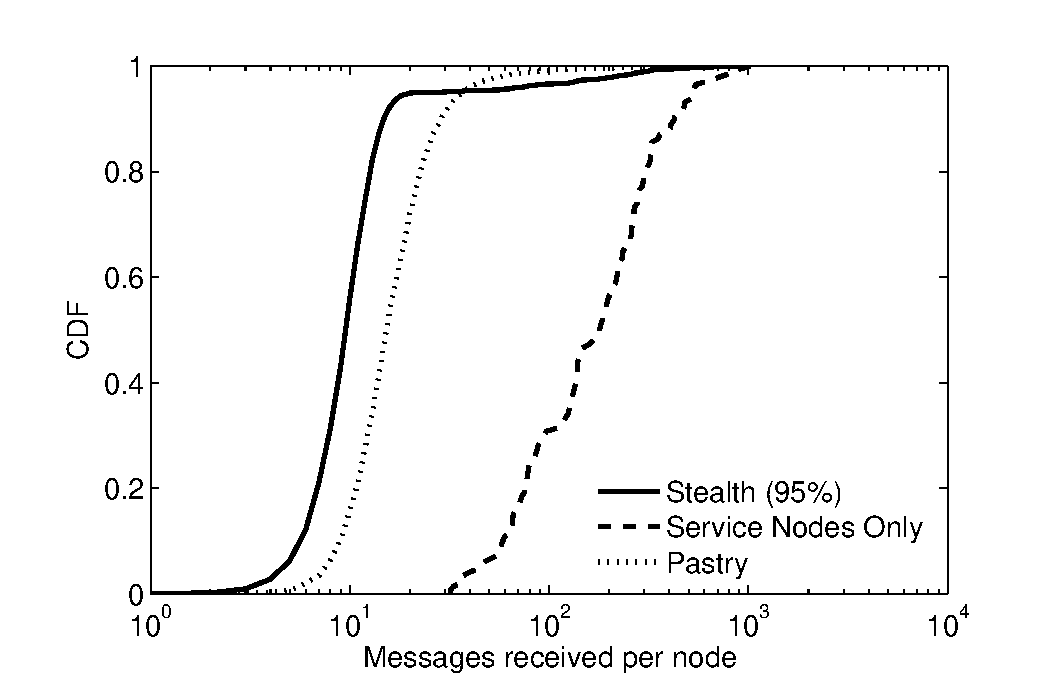
\includegraphics[width=0.415\textwidth]{./diagrams/recv_per_node}
    \label{fig:messagespernode}}
\subfigure[{\em With Churn}]
    % generated by plotpacketsperlink.m
    % workload is KeysChurnTest (Normal and Stealth (95%))
    {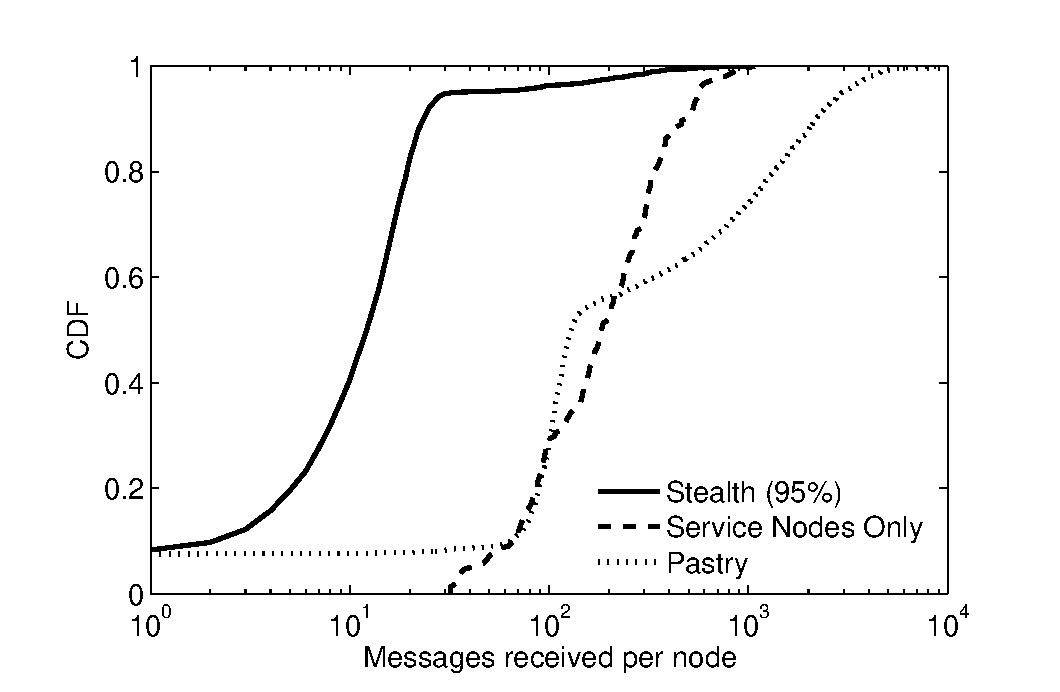
\includegraphics[width=0.415\textwidth]{./diagrams/recv_per_node_churn}
    \label{fig:messagespernodec}}
\caption{\em Distribution of received messages per node}
\label{fig:messages}
\end{figure}

Figs.~\ref{fig:messages} show the cumulative distribution function
(CDF) of received messages per node both with and without churn for
Pastry, a Stealth DHT with 95\% stealth nodes, and the Stealth DHT's
service nodes alone. We first note that the distribution of messages
per node for the Stealth DHT exhibits the same expected non-uniformity
for the network both with and without churn with only 5\% of the nodes
handling between 20 and 1,000 messages, and 95\% of nodes receiving
less than or equal to only 20 messages. In this simulation, only
stealth and Pastry nodes churned. The CDF of received messages per
service node is also shown on the figure, showing a slightly more
uniform distribution for received messages for service nodes than for
all nodes. This shows that a Stealth DHT retains the ability to balance
load amongst its service nodes.

In contrast with the Stealth DHT, Figs.~\ref{fig:messages} also show
that the distribution of messages for Pastry without churn differs from
that with churn. For the case without churn, the CDF of messages shows
a gentler slope and a smoother curve than for the Stealth DHT, with
Pastry nodes receiving between around 1 to 1,000 messages, as with the
Stealth DHT. The steepness of the curve indicates the expected uniform
distribution of messages amongst the nodes for Pastry. As seen in
Fig.~\ref{fig:messagespernodec}, the distribution of messages among
nodes in Pastry {\em under churn} is, unexpectedly, not uniform. We
observe that the variation of messages per node is significantly higher
for Pastry between 1 and $10^4$ compared to 30 and $10^3$ for service
nodes. Thus, under churn service nodes actually experience less load
than a typical Pastry node due to the fewer maintenance messages
required.

\begin{figure}[tb]\centering
\center \subfigure[{\em Without Churn}]
    % generated by plotcdfrecv.m
    % workload is KeysChurnTest (Normal and Stealth (95%))
    {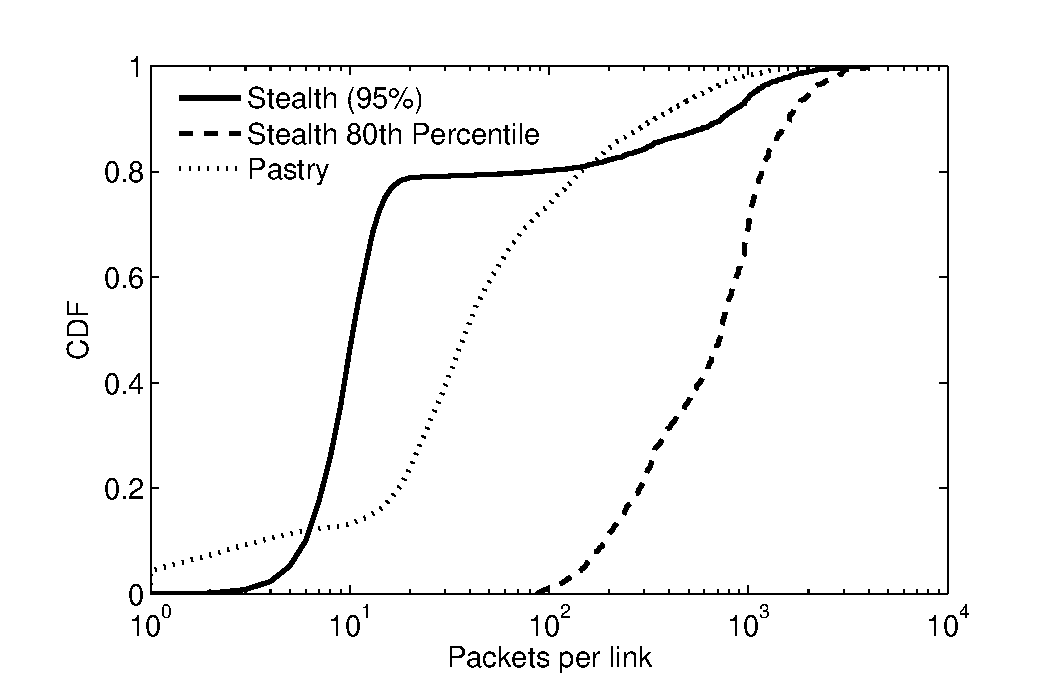
\includegraphics[width=0.415\textwidth]{./diagrams/packets_per_link}
    \label{fig:packetsperlink}}
\subfigure[{\em With Churn}]
    % generated by plotpacketsperlink.m
    % workload is KeysChurnTest (Normal and Stealth (95%))
    {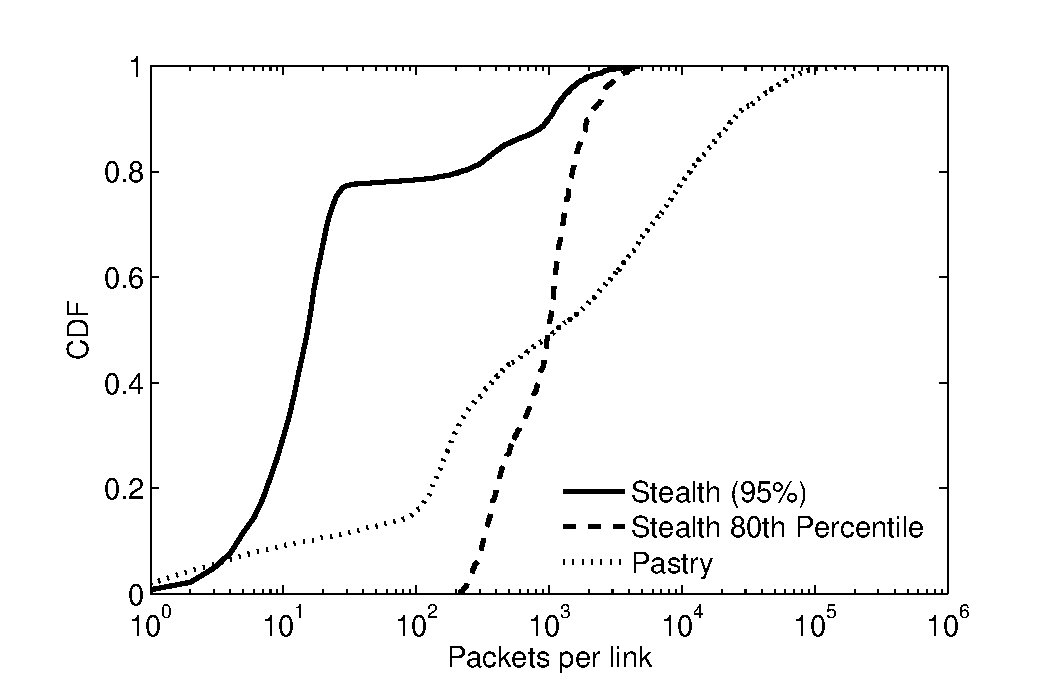
\includegraphics[width=0.415\textwidth]{./diagrams/packets_per_link_churn}
    \label{fig:packetsperlinkc}}
\caption{\em Distribution of packets per link (Stress)}
\label{fig:packets}
\end{figure}

Figs.~\ref{fig:packets} show the CDFs of packets per physical link for
Pastry, a Stealth DHT with 95\% stealth nodes, and the $80^\mathrm{th}$
percentile of links in a Stealth DHT, for cases with and without churn.
Packets per link is also known as link {\em stress}. Similar trends to
Figs.~\ref{fig:messages} are shown for both Pastry and a Stealth DHT
when there is no churn. Expectedly, around 80\% of the links in the
Stealth DHT handle less than or equal to 20 packets, and the remaining
20\% of links handle between 20 and $4~\times~10^3$ packets. The
resultant performance is near-identical regardless of churn. Of
interest is the stress performance difference between Pastry with and
without churn. We observe from Fig.~\ref{fig:packetsperlinkc} that
under churn, the distribution of packets per link in Pastry varies
highly, causing a small percentage of links to handle significantly
more packets compared to when there is no churn.

To verify that no link was uniquely overloaded in the Stealth DHT, we
plotted the CDF of packets for the $80^\mathrm{th}$ percentile of
packets per link, which is observed to be quite uniform and  unaffected
by churn (see Figs.~\ref{fig:packets}).

\begin{figure}[tb]\centering
\center \subfigure[{\em Without churn}]
    % generated by plotcdfrecv.m
    % workload is KeysChurnTest (Normal and Stealth (95%))
    {\includegraphics[width=0.415\textwidth]{./diagrams/stress}
    \label{fig:stressnc}}
\subfigure[{\em With Churn}]
    % generated by plotpacketsperlink.m
    % workload is KeysChurnTest (Normal and Stealth (95%))
    {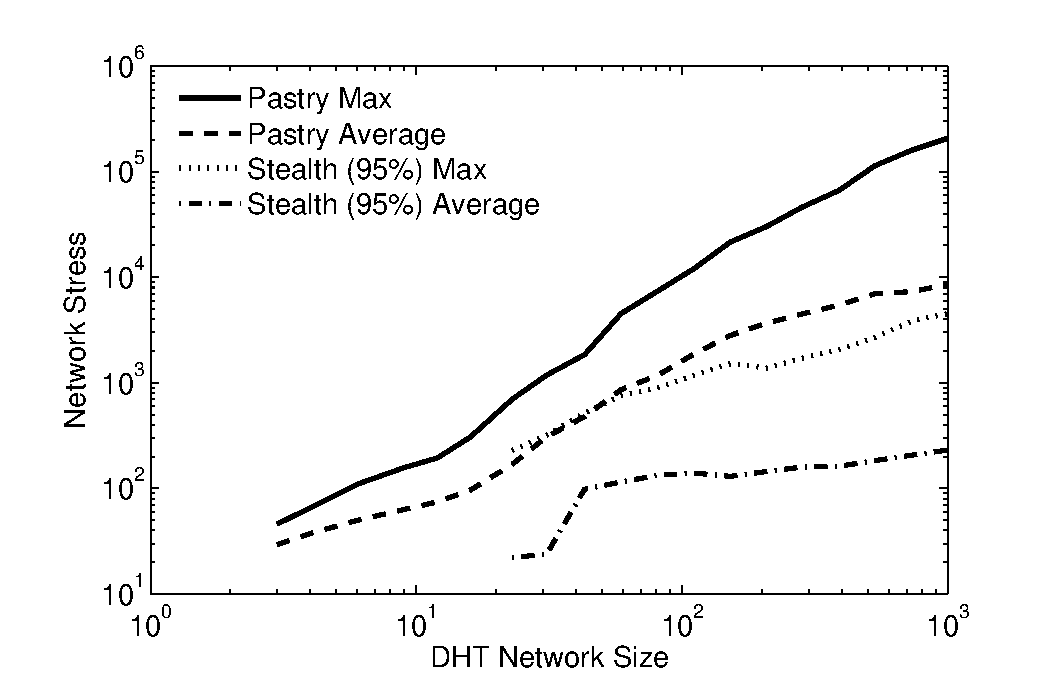
\includegraphics[width=0.415\textwidth]{./diagrams/stress_churn}
    \label{fig:stressc}}
\caption{\em Number of packets handled per link as a function of
network size} \label{fig:stress}
\end{figure}

We further compared the performance of Pastry and a Stealth DHT with
95\% stealth nodes in terms of the average and maximum stress as a
function of network size, both with and without churn. These results
are shown in Figs.~\ref{fig:stress}. Expectedly, links in the
Stealth DHT experience higher average and maximum  stress
performances than links in Pastry when there is no churn. This is
because packets in a Stealth DHT are more likely to follow  similar
paths than in Pastry due to a smaller number of routing service
nodes (only 5\% of all nodes).

Fig.~\ref{fig:stressc} shows the stress performance under churn. The
results show that links under Pastry experience much higher average and
maximum stress than links in the Stealth DHT. Take a network of 1,000
nodes for example, Pastry results in average and maximum stress of
$10^4$ and $2~\times~10^5$ compared to average and maximum stress for
the Stealth DHT of only 200 and $4~\times~10^3$ respectively.

To sum up, Figs.~\ref{fig:messages} and Figs.~\ref{fig:packets} show
that Pastry under churn distributes load less effectively between its
nodes than a Stealth DHT does amongst its service nodes. Whereas
Figs.~\ref{fig:stress} shows that Stealth DHTs lead to higher maximum
stress than Pastry, while actually providing lower average and maximum
stresses when under churn. We attribute the unbalanced load and the
increase stresses in Pastry to the many messages generated when a node
churns. The combination of the \emph{join} and the \emph{announcement}
messages causes each Pastry node to see approximately an order of
magnitude more messages than a Pastry node not under churn. Since
stealth node on the other hand do not use \emph{announcement} messages,
service nodes see much less messages than their Pastry counterparts.

\subsubsection{The Effect of Increasing Churn}
\label{subsubsect-churn}

While we assume that service nodes are stable machines, it is
important to know what to expect if, for some reason, they become
unstable. We therefore examined how a Stealth DHT with 95\% stealth
nodes performed under increasing levels of churn.

\begin{figure}[tb]
\centering
\epsfig{file=./diagrams/IncreasingChurnStealthRep,width=0.415\textwidth}
\caption{\em Percentage of misses under decreasing churn}
\label{fig:increasechurnstealth}
\end{figure}

Fig.~\ref{fig:increasechurnstealth} shows the percentage of misses as a
function of decreasing churn rate. From the figure we can see that as mean
inter-arrival/departure time decreases, the percentage of misses increases
steadily, climbing increasingly rapidly for the highest rates of churn. It is
also clear from the figure that regardless of the rate of churn, replication
provides a significant improvement in key availability.

\subsubsection{Improvement Over Random Selection}
\label{subsubsect-random}

\begin{figure}[tb]\centering
\subfigure[Percentage increase in end-to-end latency]
    {\includegraphics[width=0.415\textwidth]{./diagrams/RandomNodeLatIncrease}
    \label{fig:randomlat}}
\subfigure[Number of messages received per service node]
    {\includegraphics[width=0.415\textwidth]{./diagrams/RandomNodeStressLog}
    \label{fig:randomstress}}
\caption{\em Comparison between the use of a single row routing table and
random selection} \label{fig:random}
\end{figure}

As mentioned in Section~\ref{subsect-state}, one may argue that the complexity
of using a routing table with a single row is unnecessary, if randomly
selecting a first hop from a set of $2^b$ randomly obtained service nodes
offers similar performance. However, by simulating both scenarios with 1,000
nodes (95\% stealth) we show that this is not the case.

Fig.~\ref{fig:randomlat} shows the percentage increase in end-to-end latency
when randomly selecting a first hop relative to using a single row routing
table. Clearly, we observe that both approaches exhibit similar performance for
small networks (fewer than 20 nodes), whereas as network size increases above
20, we see that a random selection results in higher latencies with increasing
discrepancy as a function of network size. For example, for a network of 1,000
nodes, a random selection produces a 30\% increase in end-to-end latency.

The improved performance observed for a single row routing table is due to the
fact that the first hop under random selection makes little or no progress
towards the message destination. In particular, while DHT paths are made up of
a series of hops of exponentially decreasing length, the first random hop
potentially adds a long hop to the path; thus seriously degrading the quality
of the overall end-to-end path.

Fig.~\ref{fig:randomstress} shows the CDF of messages received per service node
for both scenarios. We first observe that the number of messages per node is
higher if nodes select their first hop randomly. For instance, around 40\% of
the service nodes in the Stealth DHT receive fewer than 200 messages, whereas
if the first hop is randomly selected then all nodes receive more than 200.
This shows that random selection also results in a larger average number of
messages than if a single row routing table is used. The percentage of nodes
that receive a large number of messages is similar for both cases, and is
caused by the combined effect of the Zipf popularity for the keys, as used in
the simulations, and normal DHT routing behaviour. Indeed, this similarity is
to be expected, as the set of nodes chosen as the first hop in the Stealth DHT
case is the same as the set of nodes chosen as the second hop in the random
case.

\subsection{Implementation}
\label{subsect-impl}

In addition to simulations we also created and deployed an
implementation of a Pastry-based Stealth DHT onto
PlanetLab~\cite{planetlab}. This section compares the performance of
Stealth DHT to that of Pastry while running on a real-world
platform. PlanetLab provides roughly 600 nodes, but at any time
roughly only 400 of these were active. Every implementation run we
used a randomly selected set of nodes from the pool of 400. Each
node ran four instances of our implementation, thus when we have
results for 1200 nodes, this actually represents 300 physical
machines, each hosting four nodes. When we used the Stealth DHT
portion of the implementation, we randomly selected which nodes
would be service nodes and which would be stealth nodes from the
pool of available nodes. However, we ensured that at most one
instance of a service node would be run on any physical machine. The
nodes would then use a random \emph{bootstrap} node from the set of
joined service nodes, thus providing a uniformly distributed load
during join.

While using PlanetLab we encountered some limitations in the use of
our implementation, these were the common problems of timing and
unpredictable node failures. Given the number of physical nodes used
and their geographical diversity, it is perhaps to be expected that
many would have their clocks incorrectly set and/or be prone to
occasional failure. We therefore examined all retrieved data
carefully, discarding results where necessary.

\begin{figure}[tb]
\centering
\epsfig{file=./diagrams/Imp_PlotJoinsMessages_PerNode,width=0.415\textwidth}
\caption{\em Average number of messages generated per node during a single
join} \label{fig:imp_joinmsg}
\end{figure}

We first examine the overhead caused by joins. This was also looked
at within the simulator in Section~\ref{sect-join-performance}, but
in Fig.~\ref{fig:imp_joinmsg} we verify if these overheads hold true
in the real-world. Here we plot the number of messages generated on
average when a single node (service or stealth) joins the network as
a function of network size. This includes the initial join message,
the state sent back to the node and also the announcements sent back
into the network. Pastry nodes consistently generate between 30 and
50 messages for each join; the majority of these are the
announcement messages, and messages sent to nodes' leafsets. In the
case of Stealth DHTs, when a stealth node joins these announcement
and leafset messages are not generated, thus producing values
between 5 and 15 messages per join (for the considered network sizes
of 50\%, 80\% and 95\% stealth nodes).

\begin{figure}[tb]
\centering \epsfig{file=./diagrams/Imp_PlotGetHops2, width=0.415\textwidth}
\caption{\em Average DHT hops for get message in varying sized Pastry and
Stealth networks} \label{fig:imp_gethops}
\end{figure}

Fig.~\ref{fig:imp_gethops} shows the average number of hops a
\emph{get} message takes to get to its destinations for differently
sized networks. Lines of best fit are also plotted for clarity.
These results show the same trends as the simulation results, as
well as the expected results. However, in all cases they exhibit
slightly more hops than the anticipated values: 15\% for Pastry and
between 10\% and 12\% for the stealth DHT lines. These increased hop
counts can be explained by Fig.~\ref{fig:imp_failedpaths}.

\begin{figure}[tb]
\centering \epsfig{file=./diagrams/Imp_PlotFailedPaths,width=0.415\textwidth}
\caption{\em Percentage of messages that experience at least one failed hop on
their path as a function of network size} \label{fig:imp_failedpaths}
\end{figure}

While running our implementation on PlanetLab, we found that there were
a significant number of nodes with non-transitive connectivity
(\emph{i.e.} a node $A$ may be able to contact $B$, $B$ may be able to
contact $C$, but $C$ cannot contact $A$)~\cite{nontransitivity}.
Fig.~\ref{fig:imp_failedpaths} shows the percentage of messages that
experience at least one failed hop between source and destination. This
does not indicate that the message failed to be delivered, just that
the optimal path failed and a alternative route was taken. When an
alternative route is taken this adds to the end-to-end delay of the
message, as well as degrading DHT network performance. The results for
Stealth DHTs are excluded from the plot for clarity but have similar
points with similar trend lines.

\section{Applications of Stealth DHT}
\label{sect-applications}

The Stealth DHT approach has several noteworthy features that make
it appealing for a number of applications. As one might expect, any
application that can make use of a traditional DHT could also be
implemented on top of a Stealth DHT, often leveraging the additional
properties offered to provide greater functionality and performance.
The benefits, such as scalability, resilience, improved performance
and so forth should be common to all applications built upon the
Stealth DHT foundation.

A good example of where nodes may have low capabilities and a short lifetime is
a mobile environment. The nature of mobile communications means that these
nodes are particularly likely to cause churn, which causes serious problems for
traditional DHTs~\cite{mobilechurn}. It is also important that such nodes be
able to join the network quickly and efficiently, otherwise the time taken
connecting to the network may dominate their lifespan. A Stealth DHT therefore
provides an ideal solution by supporting mobile nodes as stealth nodes as
discuss in~\cite{stealthpercom}.

Commercial applications such as content delivery networks could also
make good use of a number of specific features. By using identification
and authentication (\emph{e.g.} digital certificates) in conjunction
with a Stealth DHT, a (DHT) service provider can control which
operations nodes are allowed to carry out. For example, an announcement
message (see Section~\ref{subsect-join:service}) can be discarded and
ignored by service nodes if it does not carry proper credentials,
ensuring that only authorised nodes join as service nodes. In the same
manner, a DHT service provider could control who publishes what on its
network as well as using the authentication information provided to
trace content publishers if need be, whilst being able to guarantee to
clients (stealth nodes) that they will only talk to trusted nodes
(service nodes). These are by no means an exhaustive list of the
powerful control a DHT service provider can regain through the combined
use of Stealth DHT and authentication. Such control would, in turn,
allow the service provider to repel some of the major common security
issues present in peer-to-peer networks, such as sniffing,
man-in-the-middle, pollution and some denial-of-service attacks, while
still benefiting from the scalability and resilience of these networks.
We also discuss this topic further in~\cite{stealtheuromicro}.

Certain applications may also require that the source of messages be
addressable on the DHT. As no state regarding stealth nodes is stored
in service nodes, this is impossible without an extension to the
Stealth DHT.

Recall that service nodes deliberately avoid keeping any state on
stealth nodes as a means of improving performance and security. It
is therefore important to design addressability mechanisms for
stealth nodes that do not jeopardise these basic design principles.
We propose two application-specific solutions to this issue:
\emph{Registration} and \emph{Encapsulation}.

Registration, as the name suggests, involves stealth nodes
registering their existence with the service node closest to their
IDs in the address space, by simply sending a registration message
towards their own ID. The corresponding service node can then record
the registering stealth node's ID and pertinent other details in
what we refer to as a \emph{Addressing Table}\footnote{The
information in an addressing table should be maintained using an
appropriate soft-state mechanism.}. The registration method
therefore allows the service node with which a stealth node
registered to forward the appropriately addressed DHT messages to
it. Registration information can also be used to detect collisions
between stealth node IDs (see Section~\ref{subsect-join:stealth})
and take appropriate remedial action.

In request-response circumstances, where service nodes only need to be able to
reply to stealth nodes via the DHT rather than direct unicast, then our
encapsulation method may provide a better solution. In encapsulation, the
service node which happens to be the first hop of a stealth node's message
records information about this message for a limited time, and forwards it on
as though the message was sent by the service node itself. The message also
contains a local identifier associated with the message\footnote{Original
message fields and the local identifier may be encoded as optional header
field}. Note that stealth node ID collisions may not be a problem with this
method, as the information held in message records can include differentiating
information such as the stealth nodes' IP addresses. Collisions would then be
resolved as different local identifiers.

Fig.~\ref{fig:addressability} shows the number of dependent stealth
nodes per service node for a DHT with 10,000 stealth nodes and 200
service nodes. For registration, each stealth node registered, while
for the encapsulation example, each stealth node sent a message to
the same service node. The more uniform repartition of stealth nodes
among service nodes is obviously explained by the fact that both
service and stealth nodes are uniformly distributed across the
overlay and registration information is kept at the service node
closest to the corresponding stealth node. The apparent
concentration of state on just a few service nodes in the
encapsulation case is caused by the routing strategy which, in
essence, divides the DHT ring into $2^b$ equal regions and always
strives to find a first hop within the region where the destination
lies (in our case this destination is unique). The observant reader
will have noticed that with encapsulation, service nodes outside
this restricted region also hold a small amount of encapsulation
state. This is caused by incomplete or invalid entries in some
stealth node routing tables, forcing these nodes to pick a first hop
at random.

The choice of stealth node addressability mechanism is application
dependent and the results above are provided solely to guide such a
choice.

\begin{figure}[tb]
\centering \epsfig{file=./diagrams/Addressability,width=0.415\textwidth}
\caption{\em Stealth nodes addressability: service nodes overhead}
\label{fig:addressability}
\end{figure}

\section{Related Work}
\label{sect-related}

A number of previous works have also proposed improving DHT performance
by separating network nodes into groups of more and less capable nodes,
wherein the more capable nodes are often referred to as
\emph{super-peers}. Indeed, the notion of incorporating such a strategy
into traditional DHT algorithms is seemingly similar to that of our
Stealth DHT proposal. However, we should stress that there are a number
of key differences in our approach.

Mizrak \emph{et al.}~\cite{mizrak03structured}, and Zhu \emph{et
al.}~\cite{zhu03superpeer}, suggested similar architectures that
utilised a dual overlay DHT where one overlay exists for the
super-peers, and another for the normal peers. In these approaches
peers will forward onto the super-peer overlay first via their
nearest super-peer, which continues forwarding towards the
destination super-peer. In turn the destination super-peer moves the
message back onto the normal overlay. The problem with this approach
is that each normal peer is associated with a single super-node,
which results in a single point of failure, and also requires each
super node to retain a large amount of state. In our system, stealth
nodes are connected to the DHT itself, albeit without appearing to
other nodes. The advantage of our approach is that a stealth node is
not reliant on any one service node for connectivity; in the event
of a failure, the DHT algorithm will automatically ensure that a
suitable replacement can forward any data that a stealth node wishes
to send without extra overhead. In addition, as stealth nodes decide
their own first hop we achieve slightly improved levels of routing
performance.

Xu \emph{et al.}~\cite{xu03reducing} suggest a DHT where nodes are
only added into the routing tables after the node has appeared on
the network for a given length of time. This allows the more stable
nodes to be identified and used in preference. However this
technique requires continuous probing of newly joining nodes to
calculate their stability. They claim that this additional overhead
is less than the maintenance overhead required when there is churn,
however they have left their evaluation as future work.

The topic of how churn affects DHTs has also been widely discussed. Rhea
\emph{et al.}~\cite{churn1} demonstrated how many DHT implementations simply
break under high levels of churn, especially with high levels of background
traffic. As a consequence, any attempt to use a traditional DHT with unstable
nodes (mobile clients, for example), is unlikely to yield acceptable
performance. While there have been several efforts to solve this
issue\cite{mobilechurn}, they still involve placing unstable nodes into the DHT
itself whilst using complex algorithms to attempt to lessen the effect of
churn. Our system takes a simpler approach in that as stealth nodes are not
allowed to forward data, their transient nature does not affect the routing
performance of the network.

In Section~\ref{subsect-join:stealth}, we discussed that one of the benefits
of stealth DHTs is that it is relatively inexpensive in terms of the
number of messages generated to join a stealth node to the network.
Nodes on a traditional DHT, however, often exchange substantial
numbers of messages when a new node joins. Making this process more
efficient has been discussed previously~\cite{xu03reducing}, however Li \emph{et al.}~\cite{dhtcomparison} point out that a number of DHT
studies do not look at all the parameters, such as the amount of
bandwidth consumed.

\section{Conclusions}
\label{sect-conclusions}

We have proposed a simple, yet elegant method to support super-peering in DHTs.
Our stealth DHT proposal accommodates both super-peers (service nodes) and
other peers (stealth nodes) in a single overlay structure. Furthermore, Stealth
DHTs provide for the isolation of stealth nodes, therefore avoiding numerous
security and privacy issues as well as providing non-negligible performance
improvement. Straightforward extensions to Stealth DHTs have also been shown to
support applications that may require to communicate with all peer nodes using
the overlay routing. From a scalability, resilience and robustness perspective,
a Stealth DHT exhibits the same properties as the original DHT, because stealth
nodes use the original routing mechanism to choose the first hop for their
messages on the DHT, and therefore does not exhibit single points of failures
even in the presence of service node churn, whilst preserving a direct route to
the destination. Furthermore, as service nodes actually act as fully-fledged
DHT nodes, a Stealth DHT with no stealth nodes would behave like the original
DHT.

When coupled with identification and authentication, Stealth DHTs
can confer a level of control to the super-peers that is
unprecedented in today's peer-to-peer networks. Indeed, such control
can equal that provided by traditional server-based solutions, but
without compromising the many advantages afforded by the distributed
DHT solution. In essence, the Stealth DHT concept goes a long way
towards the best of both worlds.

%This paper concentrated on the modifications required for a Stealth
%Pastry DHT, however we believe that similar simple general
%principles can be applied to other DHTs too.

%As Chord and Tapestry are both ring based DHTs, they operate in a
%similar way to Pastry. A joining node must first find its place on
%the ring; in Chord this is achieved by asking the bootstrap node for
%the joining node's predecessors and fingers. Once received, the
%joining node can announce its presence to existing nodes: this step
%would be removed if a stealth node was joining, thus ensuring the
%stealth node never appears in any finger tables. Likewise, once a
%Tapestry node has acquired a optimal neighbour map it sends
%notifications to relevant nodes: again this step can simply be
%removed when a stealth node is joining. In CAN, the address space is
%split into a $d$-dimensional Cartesian coordinate space, where each
%node owns a region of this space. When a new node joins it finds the
%node owning the region where the joining node's ID would exist. This
%region is then split and the neighbours of this region are updated.
%Again, to allow a stealth node to join would simply require the last
%step of splitting the region and updating the neighbour to be
%ignored.

Finally, despite their simplicity, the principles underlying Stealth
DHT can be seen as a major enabler of more commercial exploitation
of DHT technology, therefore unleashing the true potential of
structured peer-to-peer technologies.

\bibliographystyle{abbrv}
\bibliography{conext}

\end{document}
